\documentclass[12pt]{book}
\usepackage{fontspec}
\setmainfont{TeX Gyre Pagella}
\usepackage[paperwidth=8in,paperheight=8in,margin=0.6in]{geometry}
\usepackage{xcolor}
\usepackage{amssymb}
\usepackage{amsmath}
\usepackage{tikz}
\usetikzlibrary{arrows.meta}
\pagestyle{empty}
\setlength{\parindent}{0pt}

\newcommand{\artnote}[1]{{\color{gray!70}\small\itshape [Illustration: #1]}\par\vspace{0.3in}}
\newcommand{\bigline}[1]{{\Huge #1}\par}
\newcommand{\pagenum}[1]{\vfill{\color{gray!50}\footnotesize #1}}
\newcommand{\sprollpage}{\newpage\vspace*{0.4in}}
\newcommand{\circdot}[1]{\draw[line width=2.5pt, #1] (0,0) circle (0.28in);}
\newcommand{\tridot}[1]{\draw[fill=orange!60, #1] (-0.28,-0.28) -- (0,0.28) -- (0.28,-0.28) -- cycle;}

\begin{document}

% ============ FRONT COVER ============
\thispagestyle{empty}
\begin{center}
\vspace*{1.1in}
{\Huge \textbf{SPROLL 02}}\\[0.4in]
{\huge \textbf{What Happened First?}}\\[0.5in]
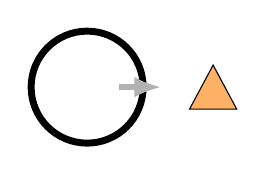
\begin{tikzpicture}
\draw[line width=2.5pt] (-0.8,0) circle (0.28in);
\draw[fill=orange!60] (0.5,-0.28) -- (0.8,0.28) -- (1.1,-0.28) -- cycle;
\draw[-{Latex[length=3.5mm]}, line width=2pt, gray!60] (-0.4,0) -- (0.15,0);
\end{tikzpicture}
\\[0.5in]
{\large \textit{order and the growing history}}\\[0.3in]
{\small The Sproll Curriculum $\cdot$ Cycle I: Pops}
\end{center}

% ============ PAGE 2: half-title / indicia ============
\sprollpage
\begin{center}
\vspace*{1.5in}
{\Large The Sproll Curriculum}\\[0.2in]
{\normalsize Cycle I --- Pops: Things, Differences, and Counting}\\[0.6in]
{\small Sproll 02 of 40 \quad $\cdot$ \quad follows Sproll 01: Something Happened}
\end{center}
\pagenum{2}

% ============ PAGE 3 ============
\sprollpage
\begin{center}
\vspace*{0.7in}
\artnote{a bold, solid circle alone on the page}

\begin{tikzpicture}
\draw[line width=3.5pt, fill=black!10] (0,0) circle (0.3in);
\end{tikzpicture}
\vspace{0.4in}
\bigline{Pop the circle.}
\end{center}
\pagenum{3}

% ============ PAGE 4 ============
\sprollpage
\begin{center}
\vspace*{0.7in}
\artnote{the same circle, now settled and plain, with a new bold triangle appearing beside it}
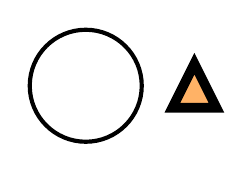
\begin{tikzpicture}
\draw[line width=1.5pt] (-0.7,0) circle (0.28in);
\draw[fill=orange!60, line width=3.5pt] (0.4,-0.28) -- (0.68,0.28) -- (0.96,-0.28) -- cycle;
\end{tikzpicture}
\vspace{0.4in}
\bigline{Then Pop the triangle.}
\end{center}
\pagenum{4}

% ============ PAGE 5 ============
\sprollpage
\begin{center}
\vspace*{0.7in}
\artnote{the circle and triangle sitting together, both plain and settled, no longer highlighted}
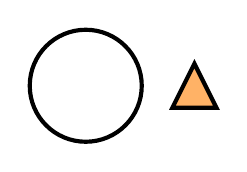
\begin{tikzpicture}
\draw[line width=1.5pt] (-0.7,0) circle (0.28in);
\draw[fill=orange!60, line width=1.5pt] (0.4,-0.28) -- (0.68,0.28) -- (0.96,-0.28) -- cycle;
\end{tikzpicture}
\vspace{0.4in}
\bigline{Here is what we have now.}
\end{center}
\pagenum{5}

% ============ PAGE 6 ============
\sprollpage
\begin{center}
\vspace*{0.8in}
\artnote{a clean, empty page -- a fresh start}
{\color{gray!40}\Huge (a clean page)}
\vspace{0.4in}
\bigline{Let's do it again, the other way.}
\end{center}
\pagenum{6}

% ============ PAGE 7 ============
\sprollpage
\begin{center}
\vspace*{0.7in}
\artnote{a bold, solid triangle alone on the page}

\begin{tikzpicture}
\draw[fill=orange!60, line width=3.5pt] (-0.3,-0.3) -- (0,0.3) -- (0.3,-0.3) -- cycle;
\end{tikzpicture}
\vspace{0.4in}
\bigline{Pop the triangle.}
\end{center}
\pagenum{7}

% ============ PAGE 8 ============
\sprollpage
\begin{center}
\vspace*{0.7in}
\artnote{the same triangle, now settled and plain, with a new bold circle appearing beside it}
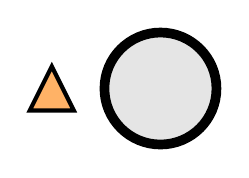
\begin{tikzpicture}
\draw[fill=orange!60, line width=1.5pt] (-0.96,-0.28) -- (-0.68,0.28) -- (-0.4,-0.28) -- cycle;
\draw[line width=3.5pt, fill=black!10] (0.7,0) circle (0.28in);
\end{tikzpicture}
\vspace{0.4in}
\bigline{Then Pop the circle.}
\end{center}
\pagenum{8}

% ============ PAGE 9 ============
\sprollpage
\begin{center}
\vspace*{0.7in}
\artnote{the triangle and circle sitting together, both plain and settled -- arranged to look exactly like the picture on page 5}
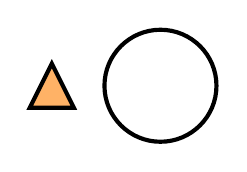
\begin{tikzpicture}
\draw[line width=1.5pt] (0.7,0) circle (0.28in);
\draw[fill=orange!60, line width=1.5pt] (-0.4,-0.28) -- (-0.68,0.28) -- (-0.96,-0.28) -- cycle;
\end{tikzpicture}
\vspace{0.4in}
\bigline{Here is what we have now.}
\end{center}
\pagenum{9}

% ============ PAGE 10 ============
\sprollpage
\begin{center}
\vspace*{0.5in}
\artnote{the two final pictures from page 5 and page 9 shown side by side, drawn identically}

\begin{tikzpicture}
\draw[line width=1.5pt] (-2.3,0) circle (0.25in);
\draw[fill=orange!60, line width=1.5pt] (-1.75,-0.25) -- (-1.5,0.25) -- (-1.25,-0.25) -- cycle;
\node at (-1.75,-0.7) {\small Picture One};
\draw[line width=1.5pt] (1.75,0) circle (0.25in);
\draw[fill=orange!60, line width=1.5pt] (1.25,-0.25) -- (1.5,0.25) -- (1.75+0,-0.25) -- cycle;
\node at (1.5,-0.7) {\small Picture Two};
\end{tikzpicture}
\vspace{0.4in}
\bigline{Are these the same?}
\end{center}
\pagenum{10}

% ============ PAGE 11 ============
\sprollpage
\begin{center}
\vspace*{0.8in}
\artnote{the same two pictures, unchanged, now with a small equals sign drawn faintly between them}
{\Huge \textbf{Yes.}}
\vspace{0.15in}\\
{\Large They look exactly the same.}
\end{center}
\pagenum{11}

% ============ PAGE 12 ============
\sprollpage
\begin{center}
\vspace*{0.6in}
\artnote{one of the two identical final pictures, alone, with a small question mark hovering above it}
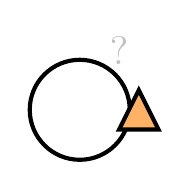
\begin{tikzpicture}
\draw[line width=1.5pt] (-0.35,0) circle (0.25in);
\draw[fill=orange!60, line width=1.5pt] (0.15,-0.25) -- (0.4,0.25) -- (0.65,-0.25) -- cycle;
\node[gray!50] at (0.15,0.75) {\Large ?};
\end{tikzpicture}
\vspace{0.4in}
\bigline{But which happened first?}
\vspace{0.15in}
{\Large The picture doesn't say.}
\end{center}
\pagenum{12}

% ============ PAGE 13 ============
\sprollpage
\begin{center}
\vspace*{0.35in}
\artnote{two small ledger strips stacked, exactly like the ones from Sproll 01 -- the top strip reads circle then triangle in that order, the bottom strip reads triangle then circle in that order}
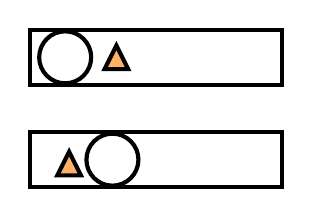
\begin{tikzpicture}
\draw[line width=1.5pt] (-1.6,0.55) rectangle (1.6,1.25);
\draw[line width=1.5pt] (-1.15,0.9) circle (0.13in);
\draw[fill=orange!60, line width=1.5pt] (-0.65,0.75) -- (-0.5,1.05) -- (-0.35,0.75) -- cycle;
\draw[line width=1.5pt] (-1.6,-0.75) rectangle (1.6,-0.05);
\draw[fill=orange!60, line width=1.5pt] (-1.25,-0.6) -- (-1.1,-0.3) -- (-0.95,-0.6) -- cycle;
\draw[line width=1.5pt] (-0.55,-0.4) circle (0.13in);
\end{tikzpicture}
\vspace{0.25in}
\bigline{The history remembers.}\vspace{0.1in}
{\Large Even when the picture doesn't.}
\end{center}
\pagenum{13}

% ============ PAGE 14 ============
\sprollpage
\begin{center}
\vspace*{0.8in}
\artnote{no new image; the two ledger strips from the previous page, shown small and quiet at the bottom of an otherwise empty page}
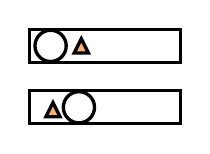
\begin{tikzpicture}[scale=0.6]
\draw[line width=1.2pt] (-1.6,0.55) rectangle (1.6,1.25);
\draw[line width=1.2pt] (-1.15,0.9) circle (0.13in);
\draw[fill=orange!60, line width=1.2pt] (-0.65,0.75) -- (-0.5,1.05) -- (-0.35,0.75) -- cycle;
\draw[line width=1.2pt] (-1.6,-0.75) rectangle (1.6,-0.05);
\draw[fill=orange!60, line width=1.2pt] (-1.25,-0.6) -- (-1.1,-0.3) -- (-0.95,-0.6) -- cycle;
\draw[line width=1.2pt] (-0.55,-0.4) circle (0.13in);
\end{tikzpicture}
\vspace{0.3in}
{\Huge \textbf{Same things.}}\\[0.15in]
{\Huge \textbf{Different history.}}
\end{center}
\pagenum{14}

% ============ PAGE 15 (closing / hand-off) ============
\sprollpage
\begin{center}
\vspace*{0.6in}
\artnote{the final picture from page 5/9 once more, plain and alone, with the same faint question mark from page 12}
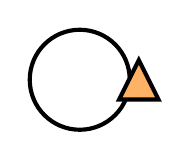
\begin{tikzpicture}
\draw[line width=1.5pt] (-0.35,0) circle (0.25in);
\draw[fill=orange!60, line width=1.5pt] (0.15,-0.25) -- (0.4,0.25) -- (0.65,-0.25) -- cycle;
\end{tikzpicture}
\vspace{0.35in}
\bigline{If the picture can't tell us,}\vspace{0.1in}
{\Large how could we ever know what really happened?}
\vspace{0.4in}\\
{\small \textit{--- turn the page for Sproll 03: Play It Again ---}}
\end{center}
\pagenum{15}

% ============ PAGE 16: Note for Grown-Ups (backmatter) ============
\sprollpage
\vspace*{0.3in}
{\large \textbf{A Note for Grown-Ups}}
\vspace{0.2in}

\normalsize
This book introduces order without introducing any new primitive. A child already knows what a Pop is from Sproll 01; this book asks what changes when two Pops happen in a different sequence.

\vspace{0.15in}
The central move is deliberately unsettling in a small, productive way: two different histories, $H_1 = \langle \text{circle}, \text{triangle} \rangle$ and $H_2 = \langle \text{triangle}, \text{circle} \rangle$, can produce the same final picture. If a child only ever looked at the resulting picture, the two histories would be indistinguishable. But the histories themselves, the ledgers of what was chosen and in what order, are not the same object, even though what they show at the end looks identical.

\vspace{0.15in}
This book does not yet explain how to recover the order from the picture alone, because in general it cannot always be done from the picture alone. That is a genuine limitation, not a simplification for children, and the curriculum returns to it formally in Sproll 07 once Collapse is available to say precisely what a picture keeps and what it discards.

\vspace{0.15in}
What this book does establish is the reason a history is worth keeping at all: a picture is already a kind of summary, and a summary can discard exactly the information that mattered. Sproll 03 takes up the natural next question raised here, whether a kept history can be trusted to reconstruct what actually happened.

\vspace{0.3in}
{\small Sproll 03: Play It Again continues directly from this book's final page.}
\pagenum{16}

\end{document}
